\subsection{Multi-node Scaling Experiments}
\label{sec:eval:theta}
\label{sec:eval:pb3}
%

%% To test the ability of \slog{} to scale structured deductive inference
%% queries to high-performance compute workloads, we implemented an
%% analysis of $k$-CFA for the $\lambda$-calculus in \slog{} and
%% evaluated its scalability on Theta~\cite{van2008deciding}.  Our
%% implementation of $k$-CFA uses a relatively standard formulation
%% similar to that in~\cite{van2008deciding}, though our presentation
%% uses the $m$-top-stack-frames interpretation giving a
%% polynomially-increasing family of analyses for a fixed sensitivity
%% $m$~\cite{might2010resolving}. We evaluated our analysis using several
%% worst-case terms we generated to systematically grow the complexity of
%% the analysis to the highest-possible number of
%% states~\cite{van2008deciding}.

\begin{wrapfigure}{R}{2.7in}
\begin{center}
\vspace{-.05in}
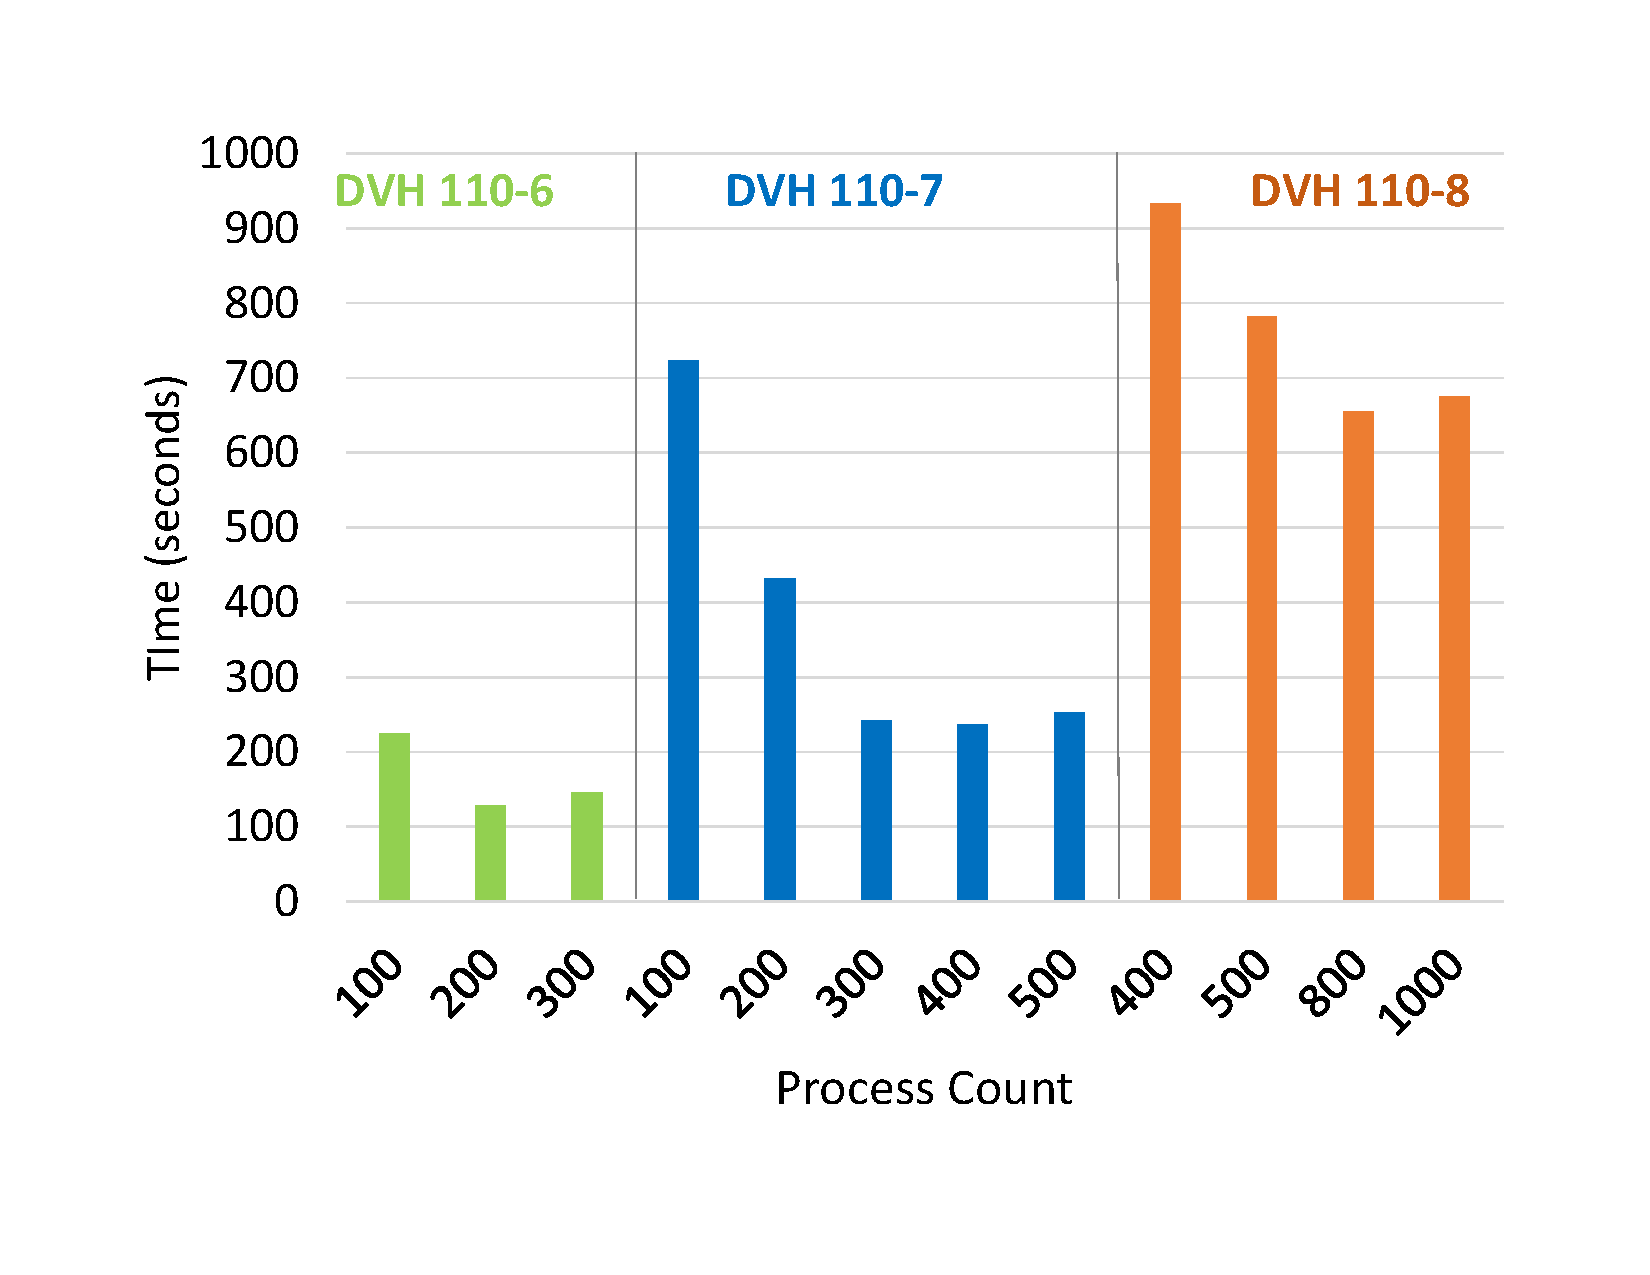
\includegraphics[width=0.5\textwidth, trim={2cm 2cm 2cm
    2cm},clip]{fig/dvh.pdf}
\end{center}
\vspace{-.15in}
\caption{Strong-scaling experiments on Theta.}
\label{fig:theta}
\vspace{-.2in}
\end{wrapfigure}

In recent years, several cloud providers have launched MPI-capabable
HPC nodes for their cloud services and significantly upgraded their
network
interconnects~\cite{azure-august2019,parallelcluster}. Alongside
related advances in cloud architectures and MPI implementations, this
move signals the ability for massively parallel analytics to be
deployed as a service in the near future. In this spirit, we also
conduct some preliminary strong-scaling experiments on the Theta
supercomputer. For this we used a fully monomorphized $m$-CFA
(distinct from the $m$-CFA used in the previous
subsection)---experiments we had ready to go when our allocation on
Theta became possible. The Theta Supercomputer~\cite{parker2017early}
at the Argonne Leadership Computing Facility (ALCF) of the Argonne
National Laboratory is a Cray machine with a peak performance of
$11.69$ petaflops. It is based on the second-generation Intel Xeon Phi
processor and is made up of 281,088 compute cores. It has an aggregate
of $843.264$ TiB of DDR4 RAM, $70.272$ TiB of MCDRAM and $10$ PiB of
online disk storage. The supercomputer has a Dragonfly network
topology uses the Lustre filesystem.


We ran three sets of $m$-CFA worst-case experiments with $110$ terms
and $m$ = $6$, $7$ and $8$. The results of the three sets of
experiments, referred to as \texttt{dvh-110-6}, \texttt{dvh-110-7} and
\texttt{dvh-110-8} are plotted in Figure~\ref{fig:theta}. For all
three set of experiments we observe improvement in performance with
increase in process counts, until maximum efficiency is attained,
after which performance degrades with increasing process counts, due
to communication overhead and workload starvation. In general, for a
given workload (problem size), we observe a range of processes that
exhibit healthy scalability. \texttt{dvh-110-6} shows a near $100\%$
scaling efficiency ($2\times$ speedup while increasing the process
count from $100$ to $200$), performance however drops when the number
of processes is increased to 300. Similarly, \texttt{dvh-110-7} shows
a $75\%$ scaling efficiency ($3\times$ speedup when the process count
is increased from $100$ to $400$), and \texttt{dvh-110-8} shows a
$71\%$ scaling efficiency ($1.42\times$ speedup going $400$ to $800$).

%Even though the largest problem is run at $2\times$ time process count,
%the scaling efficiency drops by only $4\%$, indicative of a robust and a
%scalable parallel deductive inference backend.\tom{last sentence is awful...}

